\documentclass[fr]{../../../eplsummary}
\usepackage{graphicx}
\usepackage[toc,page]{appendix} 
\usepackage{eurosym}
\usepackage{gensymb}
\usepackage{multirow}
\usepackage{chemfig}
\usepackage{tikz}
\usepackage{pgfplots}
\usepackage{pgffor}
\usepackage{qtree}

\usepackage{../../../eplchem}

\hypertitle{Projet}{3}{FSAB}{1503}
{Luca Derumier}
{Juray de Wilde}

\section{Introduction}
\par Ce document est basé sur le projet P3 de l'année académique 2016-2017, il pourrait donc ne plus être valable pour les autres années.

\section{Thématique 1 : Introduction au génie chimique}

\subsection{Procédé continu, démarrage et phase transitoire}

\par Le première thématique portait sur le laboratoire "grenadine" où nous avions dû réaliser un procédé continu qui comporte trois étape : le démarrage, la phase transitoire et le régime stationnaire.
\begin{center}
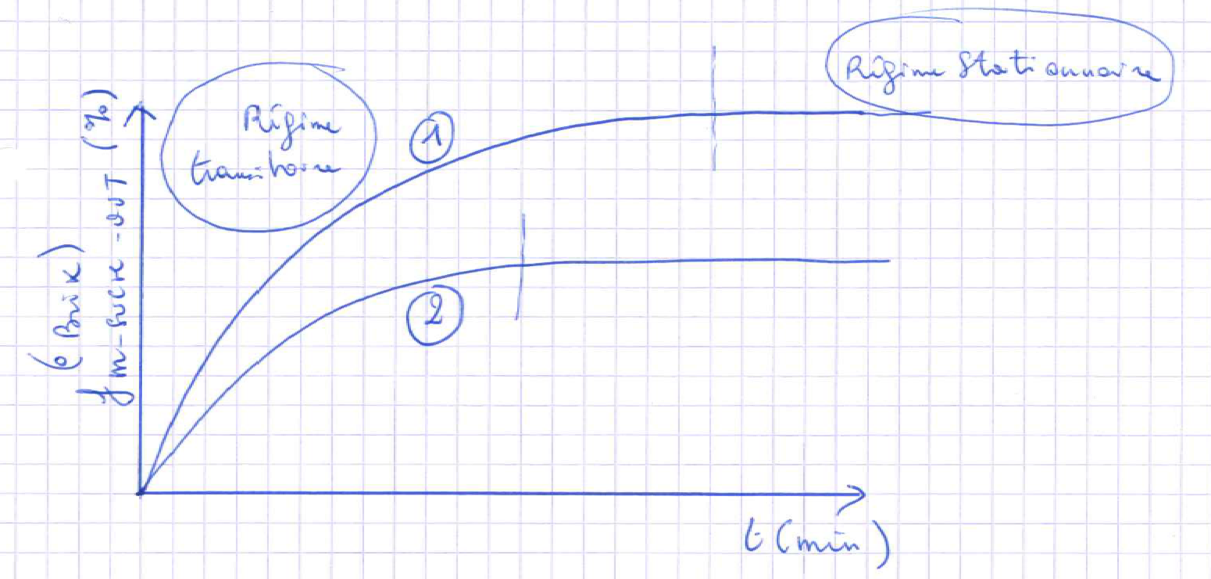
\includegraphics[scale = 0.3]{gren.png}
\end{center}

\subsection{Mesure de débits}
\par Le débit est la quantité de matière (exprimée par une masse ou un volume) qui passe à chaque unité de temps à travers cette section.

$$\dot{m} = \frac{\Delta m}{\Delta t} \,  [\frac{kg}{s}]$$

$$\dot{V} = \frac{\Delta V}{\Delta t} \,  [\frac{m^{3}}{s}]$$

\subsection{Bilan de masse}

\subsubsection{Régime stationnaire}

\par On peut vérifier le bilan de masse en régime stationnaire. Dans le cadre de la 

thématique 1 on avait :

\begin{itemize}
    \item $C_{x}$ la conentration du composant $x$ en fonction du temps en $[ \frac{kg}{L}]$ 
    \item $f_{m-x} = \frac{m_{x}}{m_{tot}}$ la fraction massique du composant $x$ dans la solution finale.
    \item $\Rightarrow C_{sucre-out} = f_{m-sucre-out} \, . \, \rho_{out}$ avec $\rho$ la masse volumique (attention à adapter les unités en fonction du problème, la masse volumique ayant les unités $[\frac{kg}{m^{3}}]$)
    \item 2 composants considérés : sucre et $H_{2}0$
    \item 2 flux entrants : Conc (Sirop Concentré) et Eau
    \item 1 flux sorant : Out\\

\end{itemize}
\par En régime stationnaire ($t=\infty$) on a donc :

$$\mbox{Débit massique entrant}=\mbox{Débit massique sortant}  $$
$$\dot{m}_{sucre-conc} = \dot{m}_{sucre-out}$$

$$\dot{V}_{conc} \, . \, c_{sucre-conc} = \dot{V}_{out} \, . \, c_{sucre-out} $$

\par On peut poser en $T=\infty$ : \\
$$\dot{V}_{in-total} = \dot{V}_{eau} + \dot{V}_{conc} = \dot{V}_{out}$$

$$\Rightarrow C_{out} = C_{sucre-conc} \, . \, \frac{\dot{V}_{conc}}{\dot{V}_{conc} + \dot{V}_{eau}}$$

$$\Leftrightarrow \frac{C_{sucre-out}}{C_{sucre-conc}} = \frac{\dot{V}_{conc}}{\dot{V}_{out}}$$

$$\Leftrightarrow \frac{f_{m-sucre-out}}{f_{m-sucre-conc}} = \frac{\dot{m}_{conc}}{\dot{m}_{out}}$$
 
\subsubsection{Phase transitoire}

\par Durant la phase transitoire, la concentration en sucre augmente dans le réacteur et donc dans le flux de sirop dilué.\\

$$C_{sucre-out} = c_{sucre-conc} \, . \, \frac{\dot{V}_{conc}}{\dot{V}_{conc} + \dot{V}_{eau}} \, . \, (1-e^{-t/\tau})$$

\par Avec $\tau = \frac{V_{R}}{\dot{V}_{out}}$ et $V_{R}$ le volume du réacteur (contenu). Si on veut vraiment se convaincre de l'origine de cette formule on peut voir qu'elle est en fait simplement la solution de l’équation différentielle suivante, qui décrit l’évolution du contenu du réacteur : 

$$\frac{\mathrm{d} C_{sucre-out}(t)}{\mathrm{d}t} = \frac{1}{V_{R}}(\dot{m}_{sucre-in}(t) - \dot{m}_{sucre-out}(t))$$
$$\Leftrightarrow \frac{\mathrm{d} C_{sucre-out}(t)}{\mathrm{d}t} = \frac{1}{V_{R}}(\dot{v}_{conc} \, C_{sucre-conc}(t) - \dot{v}_{out} \, C_{sucre-out}(t))$$

\par avec la condition limite $C_{sucre-out}(t=0) = 0$


\section{Thématique 2 : Gestion de la production}

\subsection{Réactions chimiques du projet}

\begin{itemize}
\item Combustion du méthane : $\ce{CH_{4} + 2 O_{2} \rightarrow CO_{2} + 2 H_{2}O_{(g)}}$\\
\item Vaporéformage du méthane : $\ce{CH_{4} + H_{2}O_{(g)} <=> CO + 3 H_{2}}$\\
\item Water-Gas Shift : $\ce{CO + H_{2}O_{(g)} <=> CO_{2} + H_{2}}$\\
\item Méthanation : $\ce{CO + 3H_{2} <=> CH_{4} + H_{2}O_{(g)}}$
\end{itemize}

\subsection{Equilibres chimiques simultanés et bilans de matière}

\subsubsection{Equilibre chimique global au sein d’un système}


\par Lorsque plusieurs réactions ont lieu au sein d’un même système, il en résulte, à terme, un équilibre global entre les réactifs de départ et les produits des différentes réactions, de manière à minimiser l’enthalpie libre du système.\\
\par Considérons une des réactions (appelée réaction $j$) susceptibles de se produire :

$$\ce{lL + mM <=> xX + yY}$$

\par L'enthalpie libre est minimale quand : 

$$RT \, \mathrm{ln}(\frac{(a_{X})^{x} \, . \, (a_{Y})^{y}  }{(a_{L})^{l} \, . \, (a_{M})^{m}}) = - \Delta_{r}G^{\circ \, (j)}(T)$$

\par avec $- \Delta_{r}G^{\circ \, (j)}(T)$ l'enthalpie standard molaire de la réaction $j$. La constante d'équilibre est donc : 
$$K^{(j)}(T) = \exp(\frac{- \Delta_{r}G^{\circ \, (j)}(T)}{RT})=\frac{(a_{X}^{\mbox{éq}})^{x} \, . \, (a_{Y}^{\mbox{éq}})^{y}  }{(a_{L}^{\mbox{éq}})^{l} \, . \, (a_{M}^{\mbox{éq}})^{m}}$$


\subsubsection{Calcul des concentrations après établissement de l’équilibre global du système}

\par On considère un cas particulier avec 2 réactions en phases gazeuses. On met en présence deux espèces A et B, qui sont susceptibles de réagir pour former l’espèce C, qui elle-même peut se décomposer en les espèces D et E.

\par On a donc 5 espèces en présence : A, B, C, D et E et les réactions possibles sont : 

\begin{itemize}
\item Réaction 1 : $\ce{A + B <=> C}$
\item Réaction 2 : $\ce{C <=> D + E}$
\end{itemize}

\par Après établissement de l’équilibre thermodynamique, les activités de chacune des espèces sont donc telles que :

$$K^{(1)}(T) = \frac{(a_{C})}{(a_{A})  (a_{B})} \mbox{ et } K^{(2)}(T) = \frac{(a_{D}) (a_{E})}{(a_{C})}$$


\par Lorsque le mélange est gazeux, on peut, en première approximation, égaler l’activité de l’espèce i à sa pression
partielle (en bar), ce qui permet d’écrire :\\

\begin{center}
$K^{(1)}(T) = \frac{(p_{C})}{(p_{A}) \, . \, (p_{B})}$ et $K^{(2)}(T) = \frac{(p_{D}) \, . \, (p_{E})}{(p_{C})}$ 
\end{center}

\par avec la pression partielle (en bar): $p_{i} = \frac{n_{i}}{n_{A} + n_{B} + n_{C} +n_{D} + n_{E}} \, . \, p_{tot}$\\

\par Supposons qu’on ait introduit initialement $n^{0}_{A}$ moles de A et $n^{0}_{B}$ moles de B. L’établissement de l’équilibre a nécessité que $\xi_{1}$ moles de A réagissent selon la réaction 1 et que $\xi_{2}$ moles de C se décomposent selon la réaction 2.\\ 
\par Le nombre de moles restant de chaque espèce est donc :\\
\begin{center}
\begin{tabular}{c|c|c|c|c|c|c}
     & A & B & C & D & E & Total (gaz)  \\
     \hline
     Avant réaction & $n^{0}_{A}$ & $n^{0}_{B}$ & 0 & 0 & 0 & $n^{0}_{A} + n^{0}_{B}$ \\
    \hline
    Equilibre & $n^{0}_{A} - \xi_{1}$ & $n^{0}_{B} - \xi_{1}$ & $\xi_{1} - \xi_{2}$ & $\xi_{2}$ & $\xi_{2}$ & $n^{0}_{A} + n^{0}_{B} - \xi_{1} + \xi_{2}$ \\ 
\end{tabular}
\end{center}

\par Par conséquent, les pressions partielles après établissement de l'équilbire correspondantes sont données par :

\begin{center}

A : $p_{A} = \frac{n^{0}_{A} - \xi_{1}}{n^{0}_{A} + n^{0}_{B} - \xi_{1} + \xi_{2}}\, . \, p_{tot}$\\
B : $p_{B} = \frac{n^{0}_{B} - \xi_{1}}{n^{0}_{A} + n^{0}_{B} - \xi_{1} + \xi_{2}}\, . \, p_{tot}$\\
C : $p_{C} = \frac{\xi_{1} - \xi_{2}}{n^{0}_{A} + n^{0}_{B} - \xi_{1} + \xi_{2}}\, . \, p_{tot}$\\
D : $p_{D} = \frac{\xi_{2}}{n^{0}_{A} + n^{0}_{B} - \xi_{1} + \xi_{2}}\, . \, p_{tot}$\\
E : $p_{E} = \frac{\xi_{2}}{n^{0}_{A} + n^{0}_{B} - \xi_{1} + \xi_{2}}\, . \, p_{tot}$

\par On obtient finalement : 

	\[ 
\left\{
	\begin{array}{l}
		K^{(1)}(T) = \frac{(\xi_{1} - \xi_{2})}{(n^{0}_{A} - \xi_{1})\,(n^{0}_{B} - \xi_{1})} \,.\, \frac{n^{0}_{A} + n^{0}_{B}-\xi_{1} + \xi_{2}}{p_{tot}}\\
		K^{(2)}(T) = \frac{(\xi_{1})^{2}}{(\xi_{1} - \xi_{2})}\, . \, \frac{p_{tot}}{n^{0}_{A} + n^{0}_{B}-\xi_{1} + \xi_{2}}\\

	\end{array}
	\right.
	\]	\\
	
\par On peut remarquer que les deux réactions s’influencent bien l’une l’autre car $\xi_{1}$ et $\xi_{2}$ apparaissent toutes deux dans les deux conditions d’équilibre.\\

\end{center}

\end{document}
